% \documentclass[]{template}    
% \usepackage{longtable}
% \begin{document}
\section{生成事件描述}

\subsection{本章概述}
在前两章,本文首先验证了事件描述对事件成功的影响,并通过事件属性预测了事件结果,以及衡量了事件描述与事件参与人数的关系。后者对于事件组织者尤为重要,因为一个组织者总是会关心他的活动会有多少人参加。而另一个事件组织者十分感兴趣的话题是他该如何写出好的事件描述。因此,如果能够根据历史数据,来自动生成一些事件描述供组织者参考,是十分有意义的。

本章在上一章的基础上,设计了一个生成模型(\textit{generator}),用来生成事件描述。在考察了诸多文本生成模型后,本文在本文使用了变分自编码器\cite{kingma_auto-encoding_2013,bowman_generating_2015}(\textit{variational autoencoder})。这里使用变分自编码器的原因是因为本文在设计编码器时希望文本在编码空间内服从期望的分布,具体的来说,我们希望每段文本的隐编码的周围是连续的,同时不同文本的隐编码在隐空间间也是连续的,这样的话可以避免传统编码器所带来的一些问题,比如样本在隐空间的分布不连续,导致只无法在隐空间采样来生成文本。然后本文使用上一章设计的基于GRU的神经网络作为判别器(\textit{discrimitor}),组成一个生成对抗网络\cite{goodfellow_generative_2014}。由于在训练时借鉴了强化学习中的策略梯度下降(\textit{Policy Gradient}),因此本文将其命名为GAN\_PG,通过设计合理的奖励函数,来训练生成器生成好的事件描述。

本章的结构如下:首先本文会详细介绍文本生成模型的设计和训练过程,然后本文会对GAN\_PG中使用的生成模型以及其奖励函数进行详述,最后本文会在真实的meetup数据集上给出实验结果。

\subsection{背景}
\paragraph{循环神经网络语言模型}
循环神经网络语言模型(RNNLM\cite{mikolov_rnnlm_2011})是目前十分流行的一种语言模型。在生成句子时,RNNLM仅根据当前隐层的状态给出下一个词的概率分布。而循环神经网络本身又十分强大,几乎可以拟合任何分布。而自然语言在某种程度上又可以看成一个概率模型,每一个词出现的概率都由之前已出现的词决定,因此,只要有训练数据,RNNLM就可以很好的对复杂文本序列建模。反应在实验中就是其生成的文本十分像它的训练数据,例如如果使用莎士比亚的文章作为训练数据,那么其生成文本读起来也像莎士比亚。这种性质也让它在文本生成器中得到了广泛应用,几乎所有的序列到序列(\textit{seq2seq})模型中的解码器(\textit{decoder})都采用了RNNLM。
\paragraph{变分自编码器}
RNNLM在生成文本序列中的某一个词时,完全依赖于之前输入的词和隐状态。而在实现中,通常会使用一个特殊符号来作为每一句的开头,因此,RNNLM生成的文本序列完全依赖于其刚开始时的隐状态。所以如何提供合适的隐状态来使生成的句子符合预期,就显得尤为重要了。一个解决方案是使用第二章提到的GRU编码器。编码器首先将输入序列编码到一个隐空间,然后使用一个前向神经网络将这条编码转换成RNNLM初始化的隐状态。但是这样做有一个非常明显的缺陷:无法控制输入样本经过编码器编码后在隐空间中的分布。在原空间相似的两个文本序列在编码后它们所对应的隐编码可能并不相近。这显然不是本文期望的。另一方面是,GRU在编码过程中,是直接算出对应文本序列的隐编码,而非采样获得,这就导致了隐编码在隐空间中是不连续的,换而言之,在隐空间中可能只有几个点有意义。因此,在这里仅依靠GRU编码器是不够的。但是可以通过使用变分编码器,它是传统的RNN编码器的改进型,它对隐空间中的编码\(\overrightarrow{z}\)加入了先验分布,并在目标函数中通过kl散度来缩小实际分布和先验分布的距离,以此来强迫编码器学到合适的编码方式。同时,它通过采样来生成编码,这也就保证了隐编码周围的点也都是有意义的。变分自编码器的损失函数$L_i(\theta,\phi)$如公式(\ref{3-1})。
\begin{equation}\label{3-1}
    L_i(\theta,\phi)=-E_{z\sim q_\theta(z|x_i)}[\log p_\phi(x_i|z)]+KL (q_\theta(z|x_i)||p(z))
\end{equation}

可以看出,其损失函数由两部分构成,第一部分是负对数似然损失函数NLL,用来缩小输入序列和输出序列的差异。第二个部分则是kl散度,其中$q_\theta$为编码器,$p(z)$为对隐编码$z$的先验分布。
\paragraph{生成对抗网络}
生成对抗网络(\textit{Generative Adversarial Net}\cite{goodfellow_generative_2014})是Goodfellow于2014年提出的。它包含生成(\textit{generator})模型和判别(\textit{discrimitor})模型。在训练过程中,生成模型的目标是生成能够让判别模型无法分辨出其和真实数据的区别样本,而判别模型的训练目标则是将生成模型生成的假样本从真实样本中区分开来。在标准的生成对抗网络中,本文最大化判别模型正确分类的概率,同时最小化生成模型所生成的样本被判别器正确分类的概率,目标函数见公式(\ref{3-3})。
\begin{equation}\label{3-3}
    \mathop{min}_G \mathop{max}_D V(D,G)=E_{x\sim data}[\log D(x)]+E_{x'\sim G_\theta}[\log(1-D(x')]
\end{equation}

其中,$D,G$分别表示判别和生成模型,$data$表示真实数据集。$G_\theta$表示生成模型产生的假数据。

\subsection{事件描述生成模型}
本文使用了\cite{bowman_generating_2015}中的VAE结构,如图\ref{f3-2}所示。在编码器和解码器的选择上,本文选择使用了单层GRU。在实现过程中,本文使用$0-1$高斯分布作为隐编码的先验分布。同时使用了重采样\cite{kingma_auto-encoding_2013}的技巧,这样便可以用反向传播来训练本文提出的网络:在抽样的时候,本文不直接对隐编码进行采样,而是通过两个线性神经网络获得当前编码的平均值$\bar{u}$标准差$\bar{v}$,然后通过公式(\ref{3-2})获得隐编码,其中$\bar\epsilon \sim Normal(0,1)$。
\begin{figure}[htb]\label{f3-2}
    \centering
    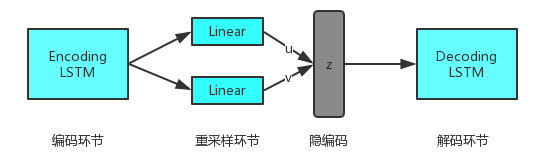
\includegraphics[width=11.3cm]{vae.png}
    \caption{事件描述生成模型的核心结构,蓝色为神经网络,灰色为向量,输入为预先训练的词向量。在编码环节完成后,LSTM的隐状态将分别输入到两个线性网络中,得到隐编码分布的平均$\bar{u}$和方差$\bar{v}$,然后通过采样获得隐编码,并将其输入解码环节。}
\end{figure}
\begin{equation}\label{3-2}
    z=\bar{u}+\bar{v}\odot \bar\epsilon
\end{equation}

至于如何使用前半段编码结果来初始化解码器中的隐状态,本文尝试了三种方法1)将隐编码连接在解码器的输入词向量的最后。2)将隐编码通过一个前向网络转换成解码器的隐状态向量,并用它直接初始化后者。3)两者皆做。在实际运用过程中,本文发现这三种方法并没有很大的差别,因此最终采用了第一种方案。

在实际的训练过程中,为了防止损失函数中KL散度降为0,本文还参考了\cite{bowman_generating_2015}中所采用的策略:在训练刚开始时设置KL散度项的权重为零,然后慢慢升到一。这样训练过程其实就分成了两个阶段:第一阶段,编码器从文本序列中学到尽可能多的信息,但不保证分布符合先验分布。第二阶段,通过增加KL散度项的权重,强迫编码器编得的隐编码尽可能接近先验分布。

\subsection{GAN\_PG}
通过前文的事件描述生成器,可以生成读上去通顺的事件描述。只要训练数据是文法通顺的句子,那么输出也会是文法通顺的句子。本文有两种方式可以获得事件描述:一种是在隐编码空间里面随机采样。这样生成的事件描述文法通顺,但无法保证语义上的一致。另一种是在已知事件描述的隐编码周围采样,由于采用了变分自编码器,相似的文本序列的隐编码在隐空间中也是相近的。因此,如果采用第二种方法,仅在已知事件描述隐编码的周围采样,便可以获得和已知事件描述在文法上相似的新的事件描述。而借助上一章的预测器,本文可以预测新的事件描述的参与人数。而通过设计合理的奖励函数,可以让解码器学到如何生成能够在预测器上获得高分的文本序列。但这样做有一个问题:我们不能保证预测器是可靠的,即在预测器上获得高分的文本序列可能并不符合我们的期望,因此在训练生成器的同时,还要对预测器进行训练,使之能正确的区分真正的样本和生成的样本,这便是此处用到生成对抗网络的原因了。
\subsubsection{GAN\_PG的结构}
GAN\_PG的生成模型为本章第二节介绍的事件描述生成模型,判别模型为上一章介绍的带GRU的神经网络。判别模型的损失函数为最小化公式(\ref{3-4})式(即在公式(\ref{3-3})前加上负号)。
\begin{equation}\label{3-4}
    \mathop{min}_D-E_{x\sim data}[\log D(x)]-E_{x'\sim G_\theta}[\log(1-D(x')]
\end{equation}
生成模型的损失函数为最大化公式(\ref{3-5})。其中$G_\theta,D_\sigma$分别为生成模型和判别模型,公式(\ref{3-5})的前半部分为在隐编码$z$和已生成的序列$y_{0:t-1}$下,生成当前$y_t$的概率。公式(\ref{3-5})的后半部分为生成模型生成$y_t$在判别模型所获得的评分。最大化公式(\ref{3-5})即最大化生成模型在生成序列的每一步中所获得的评分。
\begin{equation}\label{3-5}
pg\_loss=\mathop{min}\sum_{\substack{t}}-\log G_\theta (y_t|z,y_{0:t-1})*D_\sigma (y_t,y_{0:t-1})
\end{equation}

接下来的问题是如何衡量生成模型所生成的每一步获得的评分。因为判别模型只有在生成模型生成完整个序列以后,才能对该序列评分,而公式(\ref{3-5})所要求的是对生成序列中每一步行为的评分。在本文中,参考\cite{yu_seqgan:_2016}中所用的方法,本文使用了策略梯度来设计损失函数:对于$t$时刻所生成的序列$y_t$,本文使用了策略网络$G_\theta$(即当前生成模型)通过蒙特卡洛搜索算法对接下来$T-t$项(T为序列长)使用公式(\ref{3-6})进行采样。
\begin{equation}\label{3-6}
    \{y_0,y_1,\dotsb,y_T\}=\mathrm{MC}^{G_\theta}(y_{0:T})
\end{equation}

其中$y_{0:t}$为当前状态,$y_{t+1:T}$为基于当前生成器装态采样的结果。为了获得更准确的结果,可以将上述过程重复数次,取平均。经过改进的生成模型目标函数如公式(\ref{3-7})。
\begin{equation}\label{3-7}
Q_{G_\theta}^{D_\sigma}(y_t,y_{0:T-1})\sim 
\begin{cases}
    D_\theta(y_{0:T-1}) & \text{if } t =T-1 \\
    \mathrm{E}(D_\theta(y_{0:t-1}:y_t:y_{t+1:T-1})),y_{t+1:T-1}\sim \mathrm{MC}^{G_\theta}(y_{0:t}) & \text{if }t<T-1
\end{cases}
\end{equation}

从而$pg\_loss$便可改写为公式(\ref{3-9})。而$\nabla pg\_loss$则可以通过公式(3-10)求得。由于在计算$\nabla pg\_loss$时,判别模型的参数并不变化,所以只需要对生成模型$G_\theta (y_t|z,y_{0:t-1})$进行求导并仅更新参数$\theta$即可。本文使用公式(\ref{3-11})来更新判别模型的参数。
\begin{align}\label{3-9}
    pg\_loss &=\mathop{max}\sum_{\substack{t}}\log G_\theta (y_t|z,y_{0:t-1})*Q_{G_\theta}^{D_\sigma} (y_t,y_{0:t-1})\\
             &=\mathop{min}\sum_{\substack{t}}-\log G_\theta (y_t|z,y_{0:t-1})*Q_{G_\theta}^{D_\sigma} (y_t,y_{0:t-1})
\end{align}

\begin{align}\label{3-10}
    \nabla pg\_loss &= \nabla \sum_{\substack{t}}\log G_\theta (y_t|z,y_{0:t-1})*Q_{G_\theta}^{D_\sigma} (y_t,y_{0:t-1})\\
                    &= \sum_{\substack{t}}\nabla\log G_\theta (y_t|z,y_{0:t-1})*Q_{G_\theta}^{D_\sigma} (y_t,y_{0:t-1})\\
                    &= \sum_{\substack{t}}\nabla G_\theta (y_t|z,y_{0:t-1})*\frac{Q_{G_\theta}^{D_\sigma} (y_t,y_{0:t-1})}{G_\theta (y_t|z,y_{0:t-1})}
\end{align}

\begin{equation}\label{3-11}
    \theta \leftarrow \theta + \alpha \cdot \nabla pg\_loss
\end{equation}
在确定了判别器,生成器和其分别的目标函数后,本文通过算法一来训练GAN\_PG。
\begin{table}[htb]
    
    \centering
        \begin{tabular*}{\linewidth}{p{\linewidth}}
\toprule
            算法一、训练GAN\_PG \\
\midrule
\textbf{Require}:生成模型$G_\theta$;\\
判别模型$D_\sigma$;\\
数据集$X$;\\ 
\begin{minipage}[t]{\linewidth}
\begin{enumerate}[itemsep=-3pt]
    \item 预训练生成模型$G_\theta$
    \item 预训练判别模型$D_\sigma$
    \item \textbf{repeat}
    \item \quad \textbf{for} g-step \textbf{do}
    \item \quad \quad 使用$G_\theta$生成序列$S_{0:T}$
    \item \quad \quad 使用公式(\ref{3-10})计算目标函数
    \item \quad \quad 使用公式(\ref{3-11})更新参数$\theta$
    \item \quad \textbf{end for}
    \item \quad \textbf{for} d-step \textbf{do}
    \item \quad \quad 从$G_\theta$中\textbf{n}个负样本,从数据集$X$中抽样\textbf{m}个正样本
    \item \quad \quad 计算与目标的均方误差
    \item \quad \quad 更新参数
    \item \quad \textbf{end for}  
    \item \textbf{end for}
\end{enumerate}
\end{minipage}\\
\bottomrule
        \end{tabular*}
    \label{s3-1}
\end{table}

\subsection{训练事件描述生成模型的优化技巧}\label{train_generator}
本文提出的事件描述生成模型中的差分自编码器的目标是学会如何在隐空间中表达已有的事件描述。可以通过观察式(\ref{3-1})来判断编码的好坏:式(\ref{3-1})的前半部分,即NLL和后半部分,KL散度。一个好的编码会有相对较小的NLL和非零的KL散度。较小的NLL确保了生成结果和训练数据相似,而非零的KL散度确保了编码的相异性。但如果直接使用式(\ref{3-1})来训练,KL散度会很快降为0,即编码和先验分布完全相同了,这样便失去了编码器的意义。

当KL散度降为0时,本文提出的变分自编码器从某种程度上便和RNNLM完全相同了,前文提到,RNN可以拟合任意分布,所以在这种情况下,NLL也能降到接近0。但这样并不是本文想要的,因为如果这种情况发生,那么解码器在解码时便会完全依赖上一步生成的结果,而非编码器得到的编码。即解码器会完全忽略编码器的结果。反应在实践中,即无论输入何种文本序列,输出的文本序列都相同。

在训练事件描述生成器时,为了避免上述情况,要保证其目标函数公式(\ref{3-1})的两部分处在合适的平衡状态:NLL部分较小且KL散度较小但不为零。本文使用了两种方式来达成这一目的。

首先,本文在式\ref{3-1}的后半项增加KL系数,在训练过程中,先让后半项的系数为0,先训练前半项,再慢慢将后半项的系数增加,直到到达1为止,以训练后半项。在实现过程中,本文用了公式(\ref{3-8})来调整后半项的权重,同时为了使后半项值能稳定在合适的范围,本文将前半项的系数设置为79。

其次,本文采取的第二个措施是使用dropout层,即随机的将输入文本的某些词替换为"\_"。采用这种方式的初衷是为了弱化编码器对上一步生成的文本序列的依赖,以迫使其使用之前编码器得到的编码结果来恢复输入的文本序列。
\begin{equation}\label{3-8}
    \mathrm{KL\_Weight}=\frac{\tanh\frac{i-3000}{1000}+1}{2}
\end{equation}

\subsection{实验结果和分析}
在本小节,本文将尝试使用本章提出的生成模型来生成接近真实事件描述的文本。本文将首先从单独训练事件描述生成器入手,先用短文本进行训练,以考察变分自编码器的训练过程,及在处理自然语言中的表现。然后使用GAN\_PG进行正式训练,并考察生成的文本和真实的事件描述的接近程度。最后,本文将用训练好的GAN\_PG生成新的事件描述,以此证明GAN\_PG生成的事件描述在文法和语义上都是一致连贯的。
\subsubsection{数据集及评估指标}
本次实验使用的语料来自meetup上LA市的真实事件,具体语料信息如表\ref{t3-1}所示。在进行训练前,本文对语料库进行了如下预处理:1)去除非英文单词。2)将数字替换成“\#”。3)将出现次数少于5次的词替换为“<ukn>”。
\begin{table}[htb]
    \caption{\label{t3-1} 语料库详细信息}
    \center
    \begin{tabular*}{\linewidth}{p{.25\linewidth}p{.25\linewidth}p{.25\linewidth}p{.25\linewidth}}
    \toprule
    事件描述数量&按句划分后句子数量&平均事件描述长度&平均句子长度 \\
    \midrule 
    89924&223715&137.4&15.9 \\
    \bottomrule 
    \end{tabular*}
\end{table}

在衡量生成的事件描述的质量的时候,本文使用了\cite{papineni_bleu:_2002}作为文本质量的评估指标。BLEU起初被用于衡量机器翻译的质量,其设计思想是翻译后得到的文本与参考文本越接近越好,所以BLEU也天然适合用来衡量生成的文本与现实事件描述的接近程度。在实际实验中,本文使用了BLEU-4,即采用4-gram作为采集窗口的BLEU值。BLEU值永远在$[0,1)$之间,越接近1,则表示生成文本和参考文本越接近。

同时,为了衡量GAN\_PG的质量,本文使用了生成文本在判别模型处评分的分布与真实文本评分的分布作为衡量标准。理论上来说,一个生成模型和判别模型都处于理想状态下的GAN\_PG,为了满足纳什均衡的条件,其生成模型的评分分布一定是无限接近于真实文本的评分分布的。因此,本文选择使用评分分布的差异来衡量GAN\_PG的质量。

\subsubsection{训练事件描述生成模型}
本文使用\ref{train_generator}中提到的技巧,使用分句后的事件描述来训练事件描述生成模型,训练过程中的损失函数变化如图\ref{f3-2}所示。从图中可以看出在经历了大约120000轮的训练后,NLL和KL值都趋于稳定,最后NLL值停留在1.3附近,而KL散度停留在7附近。
\begin{figure}[htb]
    \centering
	\begin{subfigure}{.4\textwidth}
		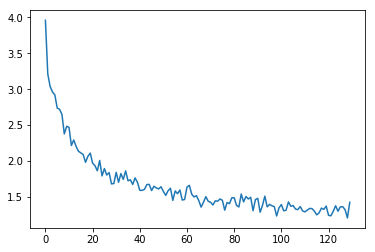
\includegraphics[width=\textwidth]{ce.png}
		\caption{前半项($\mathrm{NLL}$)变化}
	\end{subfigure}
	\begin{subfigure}{.425\textwidth}
		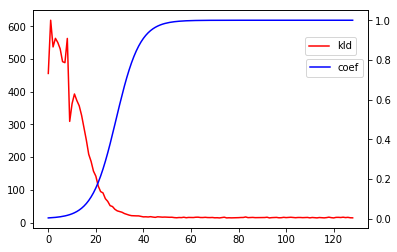
\includegraphics[width=\textwidth]{ceof.png}
		\caption{后半项($\mathrm{KL}$距离)及其系数变化}
    \end{subfigure}
    \caption{事件描述生成模型训练过程中,目标函数变化曲线,$x$轴为循环次数,最终$\mathrm{KL}$稳定在7附近}
    \label{f3-2}
\end{figure}

\paragraph{在已知样本周围采样}  
在本节中,本文将对已知样本的隐编码$z \sim \mathrm{p}(z|x)$进行采样,其中$x$为已知的文本序列,即事件描述。$\mathrm{p}(z|x)$为编码过程。本文通过公式(\ref{3-2})进行采样。通过此举,可以对生成器认为的相似的句子有个总体上的了解。实验结果如表\ref{t3-2}所示。 

\begin{table}[htb]
    \center
    \caption{\label{t3-2}对已知样本采样的结果}
    \begin{tabular*}{\linewidth}{p{0.2\linewidth}p{0.8\linewidth}}
\toprule
样本一 & we are meeting at the actual merry go round <ukn> . \\
对隐编码解码 & we will be meeting at the corner of the park entrance .\\ 
采样一 & we will be meeting in the back room , and then the <ukn> will be on the right hand side of the stage .\\
采样二 & we are going to have a great time of year 's theme for the day . \\
采样三 & we will be meeting at the end of the day before the show . \\
\midrule
样本二 & we 'll be there the whole night . \\
对隐编码解码 & we will have a dj spinning the best of the night !\\ 
采样一 & we 're going to have a great turnout .\\
采样二 & the presentation will be on the right side of the road .\\
采样三 & after the concert we 'll have a chance to visit the bars in the park . \\
\bottomrule
    \end{tabular*}
\end{table}
\paragraph{随机采样}
本节中,本文将对未知的隐编码进行采样,同时检验在编码空间中相邻点的编码结果的语义一致性和文法一致性。本文先在隐空间中进行采样,获得隐编码$z_1,z_2 \sim \mathrm{Normal}(0,1)$,然后在两点间进行线性插值,获得编码集合$\{z_i\} = t*z_1+(1-t)*z_2 ,\mathrm{for}\ t \in [0,1]$。随后再对集合$\{z_i\}$进行采样,采样结果见表\ref{t3-3}。从采样的结果可以看出,这些句子在文法上都是通畅的,且相邻的句子的语义也保持这连贯性。例如“the event is free , but donations will be greatly appreciated .”和“the event is free , but you must rsvp on meetup . ”。这也证明了本文的文本生成器的编码器学到了如何在编码的同时保持文本间语义和文法的连贯和一致性。

\begin{table}[htbp]
    \center
    \caption{\label{t3-3}随机采样结果(加粗部分为起点和终点)}
    \begin{tabular*}{\linewidth}{p{\linewidth}}
\toprule
\textbf{the event is free , but donations will be greatly appreciated .}\\
the event is free , but you must rsvp on meetup . \\
we 'll be meeting at the corner of the santa monica pier and walk to the parking lot .\\
join us for a fun evening of the evening !\\
\textbf{join us for a fun evening of dancing , fun , and fun !}\\
\midrule
\textbf{this will be a fun night to meet other people and make new friends .}\\
the event is free , but you must rsvp on meetup . \\
this is a great opportunity to meet new people and make new friends .\\
join us for a fun filled day of fun , fun and fun ! \\
\textbf{join us for a fun filled day of fun and socializing with other fun singles . }\\
\bottomrule
    \end{tabular*}
\end{table}

\subsubsection{训练GAN\_PG}
在最终的实验中,本文选择带GRU的神经网络作为判别模型,以及事件描述生成器作为生成模型。本文按照\ref{train_generator}的方法来对生成模型进行预训练,并使用最小化均方误差的方式来预训练判别模型。在正式训练时,考虑到生成模型比判别模型要难训练的多,本文设置g-step为5,d-step为1。在这里本文使用的语料库与之前几乎相同,唯一的不同是没有将事件描述拆分成句子,而是将整个事件描述输入。为了控制文本序列的长度,本文只使用了长度小于500的事件描述。
\paragraph{结果}
图\ref{f3-1}为分别训练了1,2,4个epoch后生成模型随机采样1000次产生的文本序列在判别模型获得的评价的分布与真实数据在判别模型获得评价的分布的对比,可以看出,在训练后,生成文本的评价分布更接近真实文本,这也表明了GAN\_PG的生成模型学到了如何生成高评价的文本序列,而同时其判别模型也学会了如何分辨生成文本,并且g-step和d-step的设置也比较合理。表\ref{t3-5}为预训练和训练后随机采样所生成的1000个样本的BLEU值,在这里本文采用真实文本作为参考语料库。可以看出训练后的BLEU有所提高,说明此时生成的文本更接近真实文本。
\begin{figure}[htb]
    \centering
	\begin{subfigure}{.4\textwidth}
		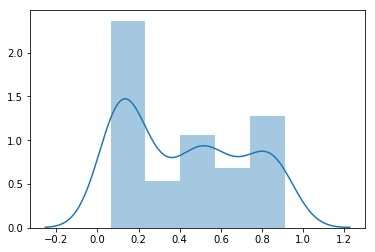
\includegraphics[width=\textwidth]{0.png}
		\caption{训练1个epoch后}
	\end{subfigure}
%%%%%%%%%%%%%%
	\begin{subfigure}{.4\textwidth}
		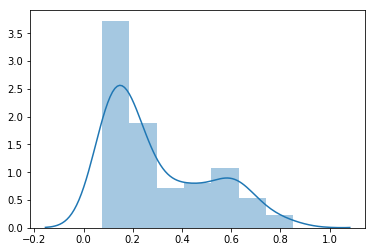
\includegraphics[width=\textwidth]{1.png}
		\caption{训练2个epoch后}
    \end{subfigure}
    \begin{subfigure}{.4\textwidth}
		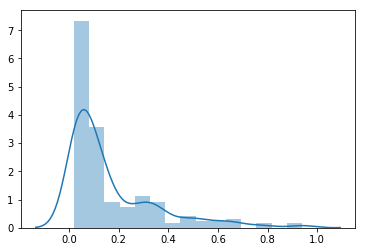
\includegraphics[width=\textwidth]{5.png}
		\caption{训练4个epoch后}
    \end{subfigure}
    \begin{subfigure}{.4\textwidth}
		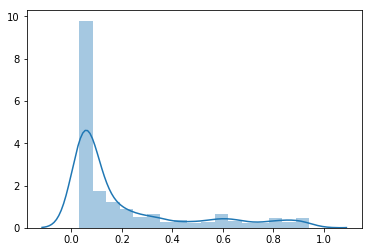
\includegraphics[width=\textwidth]{raw.png}
		\caption{真实文本的评分分布}
	\end{subfigure}
    \caption{经过数轮训练后生成序列的评分分布的变化,可以看出其越来越接近真实文本的分布}
    \label{f3-1}
\end{figure}

\begin{table}[htb]
    \center
    \caption{\label{t3-5}随机采样获得的文本序列的BLEU-4值}
    \begin{tabular*}{\linewidth}{p{.33\linewidth}p{.33\linewidth}p{.33\linewidth}}
\toprule
&预训练结束后&训练4个epoch后\\
\midrule
BLEU-4&0.64&0.67\\
\bottomrule
    \end{tabular*}
\end{table}

\subsubsection{生成新的事件描述}
在完成训练后,本文采用GAN\_PG中的生成模型来生成新的事件描述。由于使用了变分自编码器,只需要在隐空间中进行服从0-1高斯分布的随机采样便可以借助生成模型中的解码器来获得新的事件描述。为了减少随机性,我们还可以使用束搜索来最大化当前文本序列出现的概率。表\ref{t3-4}为部分随机采样下生成的新的事件描述。可以看出其文法是通顺的,并且语义也是连贯的。

\subsection{本章小结}
本章采用了变分自编码器作为生成模型,以及上一章提出的带GRU的神经网络作为判别模型,组成了GAN\_PG。实验证明,经过训练后,GAN\_PG可以较好的生成文法通畅的事件描述,并且生成事件描述的评价分布也与真实的事件描述类似,且其BLEU-4值证明了它与真实事件描述是相似的。

% \begin{table}[htb]
    % \centering
\begin{longtable}{p{.1\linewidth}p{.85\linewidth}}
\caption{\label{t3-4}随机采样下生成的新的事件描述}\\
\toprule
采样&样本\\
\midrule
\endhead
\bottomrule
\endfoot
采样一& what we \'ll do thinking about ? we \'ll see you next time. : ) join us for our weekly meet up to <ukn> games in a row . we discuss various topics about the speaker and uses that as well as his background in the next day and drive where you are the up to host and master of mindfulness for wellness promoting energy and <ukn> \'s practice . <ukn> has space for those who don t be too early . but if you \'re a part of it . you did n't know it had started already . but in an hour and some you may even forget for things . what to bring please bring a laptop and charger to class . for those who need instruction <ukn> phoenix will be <ukn> the evening . what is the thing though there is my members . there is a wonderful alternative for all of getting possible  \\
采样二 & who does your business location . you \'re invited to join our night party in a very interesting social night . join us for an evening of fun and continuously stimulating . we \'ll be taking the fight to the other music at anytime between our every wednesday night . at <ukn> : 00pm . where : the club is opened by to your head above . keep in <ukn> and get a good view of the practice . from <ukn> : you are the good seat for your solo or group routine ! limited space , so please rsvp by and we will walk you need to figure online . this will include networking events from each other and friendly , so do n't get to know other professionals in an atmosphere where you can join us ! \\
采样三& hi all ! we 'll be meeting in santa monica , ca this event at : la works most importantly come and join us in our bachata; salsa classes. 8pm open level smooth dominican bachata by arden; erika 8pm beginner level bachata by alex; <ukn> 9pm club style salsa by arden; erika 9pm advanced salsa by alex; sarah followed by the your hottest dj astro, mixing it live ! ! !\\
\end{longtable}

% \end{document} 
